\documentclass{subfiles}

\usepackage{graphicx}
\usepackage{amsfonts}
\usepackage{amssymb}
\usepackage{amsmath}

\graphicspath{ {fisica-generale/assets/} }

\begin{document}

\section{Moti}

Il moto si può classificare in base alle quantità definite (velocità, accelerazione, raggio di curva, $\dots$).

\subsubsection{Rappresentazione intrinseca del moto}

Si possono introdurre una serie di elementi per caratterizzare il moto in modo "intrinseco", cioè indipendente dal sistema di riferimento. Il primo concetto presentato è quello della ascissa curvilinea

\subsubsection{Ascissa curvilinea}

L'ascissa curvilinea, $s(t)$, è la lunghezza della traiettoria percorsa fino al tempo $t$.

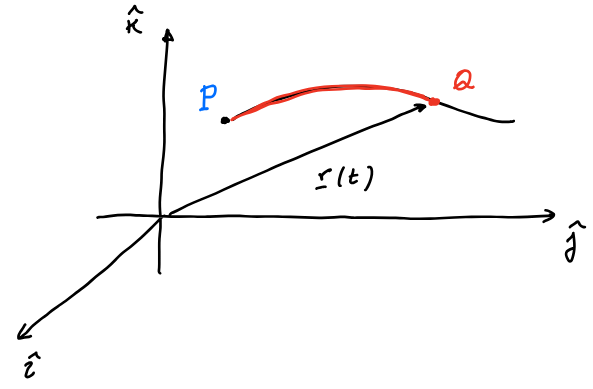
\includegraphics[width=\columnwidth]{ascissa-curvilinea}

$$
\begin{matrix}
s(t) &\simeq& \sum_{t'} |\vec{r}(t' + \Delta t) - \vec{r}(t')| \\
&\simeq& \sum_{t'} \Delta t |\vec{v}(t')| \\
&=& \int^{t}_{0}{|\vec{v}(t')| dt'}
\end{matrix}
$$

\subsection{Cerchio osculatore}

Data una curva $\vec{R}(t)$ e un punto $\vec{P} = \vec{R}(t_0)$, definiamo il cerchio osculatore come il cerchio che meglio approssima la curva vicino a $\vec{P}$.

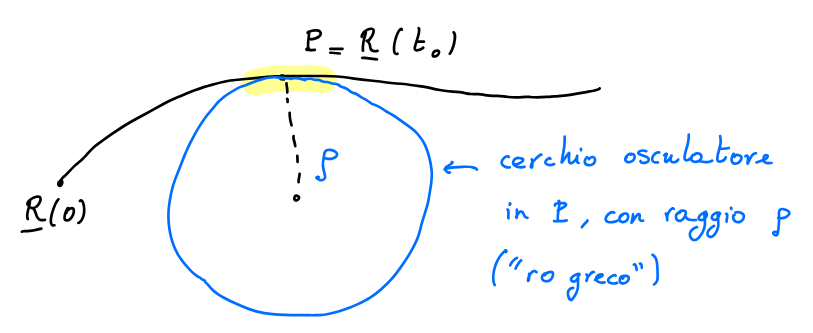
\includegraphics[width=\columnwidth]{cerchio-osculatore}

\noindent
Vicino a $\vec{P}$, la curva è indistinguibile dal cerchio blu.

\subsection{Terna vettoriale intrinseca}

Data una curva $\vec{R}(t)$ e un punto $\vec{P}$ su $\vec{R}(t)$, possiamo definire la seguente terna di versori:

\begin{description}
    \item[$\hat{u}_t$] è il versore tangente a $\vec{R}(t)$ in $\vec{P}$
    \item[$\hat{u}_n$] è il versore che punta verso il centro del raggio osculatore
    \item[$\hat{u}_b$] è il versore ortogonale a $\hat{u}_t$ e $\hat{u}_n$ ($\hat{u}_t \wedge \hat{u}_n$)
\end{description}

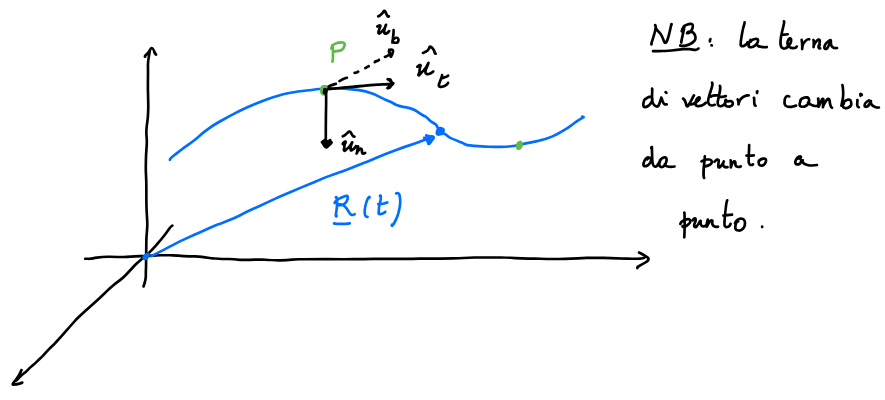
\includegraphics[width=\columnwidth]{esempio-terna-vettoriale-intrinseca}

\noindent
Si possono esprimere velocità e accelerazione in funzione della terna soprascritta.
Questa rappresentazione è utile perchè è indipendente da un sistema di riferimento fissato a priori.

\subsubsection{Velocità}

Il vettore velocità è, per definizione, parallelo a $\hat{u}_t$.

$$
\vec{v}(t) = (\frac{d}{dt} s(t)) \hat{u}_t = \dot{s}(t)\hat{u}_t
$$

\noindent
Questa equazione motiva la definizione $\dot{s}(t) =$ "velocità scalare"

\subsubsection{Accelerazione}

$$
\vec{a}(t) = \ddot{s}(t)\hat{u}_t + \frac{\dot{s}(t)^2}{\rho}\hat{u}_n
$$

\begin{description}
    \item[$\ddot{s}(t)$] "accelerazione tangenziale"
    \item[$\frac{\dot{s}(t)^2}{\rho}$] "accelerazione normale" e "centripeta"
\end{description}

\subsection{Moto rettilineo uniforme}

Un moto caratterizzato da $\vec{a}(t) = 0 \forall t$, quindi $\vec{v}(t) \implies \vec{v}$ costante $\forall t$.

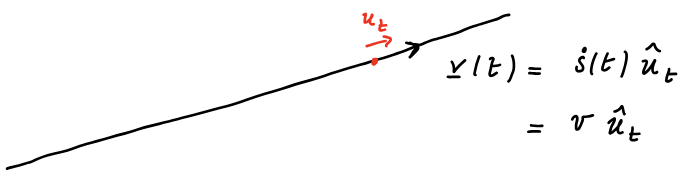
\includegraphics[width=\columnwidth]{esempio-moto-rettilineo-uniforme}

\noindent
$\dot{s}(t) = v$ costante.\\

\noindent
La legge del moto (cioè la legge che descrive $\vec{R}(t)$) è:

$$
\vec{R}(t) = \vec{R}(t_0) + (t-t_0)v\hat{u}_t
$$

\subsection{Moto uniformemente accelerato}

Un moto caratterizzato da $\vec{a}(t) = \vec{a}$ costante.
Siccome $\vec{a}$ è costante, tutto il moto si svolge su un piano.
La legge del moto è:

$$
\vec{R}(t) = \frac{1}{2}(t-t_0)^2 \vec{a} + (t-t_0) \vec{v}(t_0) + \vec{R}(t_0)
$$

\subsection{Coordinate polari}

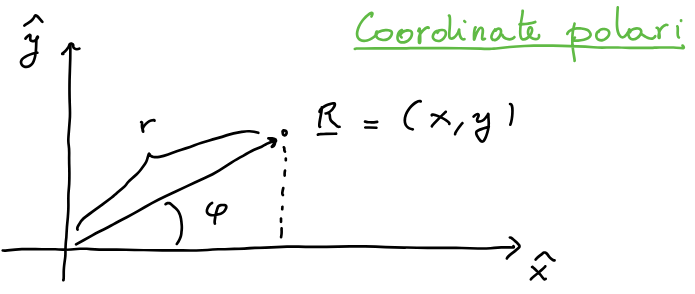
\includegraphics[width=\columnwidth]{esempio-coordinate-polari}

\begin{itemize}
    \item $r = |\vec{R}|$
    \item $\varphi$ angolo tra $\vec{R}$ e $\hat{x}$ (angolo polare)
    \item $x = r \cos{\varphi}$
    \item $y = r \sin{\varphi}$
\end{itemize}

\noindent
Con un nuovo sistema di versori $\hat{u}_r$ e $\hat{u}_\varphi$ che dipendono dal punto.

\begin{description}
    \item[$\hat{u}_r$] è lungo $\vec{R}$ e punta "all'esterno"
    \item[$\hat{u}_\varphi$] è ortogonale a $\hat{u}_r$ punta in direzione antioraria
\end{description}

\subsection{Coordinate cilindriche}

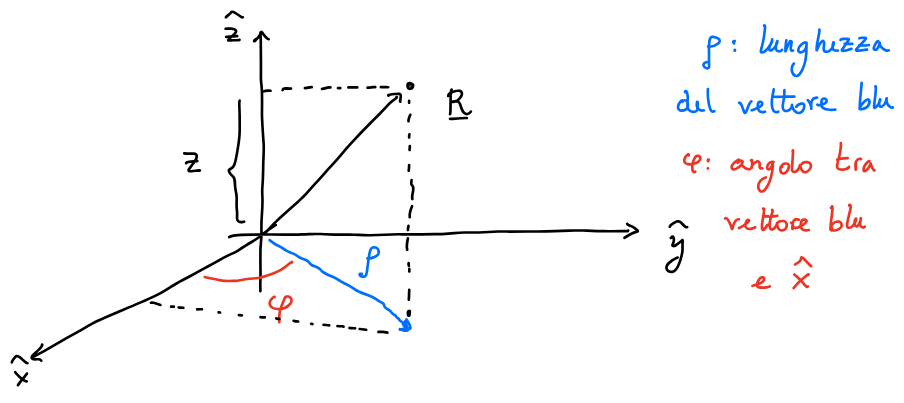
\includegraphics[width=\columnwidth]{esempio-coordinate-cilindriche}

$$
\vec{R} = (x,y,z) = (\rho \cos{\varphi}, \rho \cos{\varphi}, z)
$$

\subsection{Moto circolare}

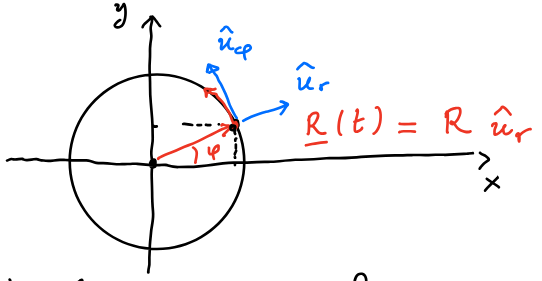
\includegraphics[width=\columnwidth]{esempio-moto-circolare}

\noindent
Moto lungo una circonferenza, è immediato vedere che $\hat{u}_\varphi = \hat{u}_t$.
Per descrivere il moto:

$$
\vec{R}(t) = R \hat{u}_r(t) = R \cos{\varphi} \hat{x} + R \sin{\varphi} \hat{y}
$$

\subsubsection{Velocità}

$$
\begin{matrix}
\dot{\vec{R}}(t) &=& -\dot{\varphi} R \sin{\varphi} \hat{x} + \dot{\varphi} R \cos{\varphi} \hat{y} \\
&=& \dot{\varphi} R (-\sin{\varphi} \hat{x} + \cos{\varphi} \hat{y})
\end{matrix}
$$

\begin{description}
    \item[$\dot{\varphi}(t)$] velocità angolare (la variazione dell'angolo polare in un piccolo intervallo di tempo).
\end{description}

\subsubsection{Accelerazione}

$$
\vec{a}(t) = R \ddot{\varphi}(t)\hat{u}_\varphi - R \dot{\varphi}(t)^2\hat{u}_r
$$

\begin{description}
    \item[$R\ddot{\varphi}$] accelerazione tangenziale
    \item[$-R\dot{\varphi}^2$] accelerazione normale o centripeta
\end{description}

\noindent
Se $R\ddot{\varphi} = 0$ parliamo di moto circolare uniforme,
dove la velocità angolare è costante ($\omega$),
ma l'accelerazione centripeta è $a_n = -R \omega^2 \neq 0$.\\

\noindent
$\varphi$ si misura in radianti (rad), $\dot{\varphi}(t)$ si misura (rad/s).

\subsection{Moti periodici}

Un moto è detto periodico con periodo $T$ se:

$$
\vec{R}(t+nT) = \vec{R}(t)
$$

\noindent
$\forall n \in \mathbb{N}$

\begin{description}
    \item[$T$] periodo
    \item[$\upsilon$] frequenza ($\frac{1}{T}$)
    \item[$\omega$] pulsazione ($\frac{2\pi}{T}$)
\end{description}

\noindent
Il moto circolare uniforme è un esempio di moto periodico

\subsubsection{Moto armonico}

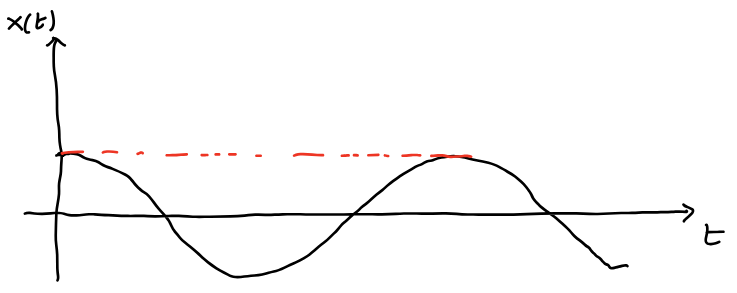
\includegraphics[width=\columnwidth]{esempio-moto-armonico}

\noindent
Un qualsiasi moto caratterizzato da una equazione differenziale del tipo:

$$
\ddot{\vec{R}}(t) = -A\vec{R}(t)
$$

\noindent
$\forall A > 0$\\

\noindent
Data $\ddot{f}(t) = -Af(t)$, la soluzione più generale è:

$$
f(t) = \alpha \sin{(\omega t + \varphi_0)}
$$

\noindent
dove $\omega = \sqrt{A}$, mentre $\alpha$ e $\varphi_0$ sono parametri liberi che vanno fissati dalle condizioni iniziali.

\end{document}
